\documentclass[10pt]{beamer}
\usetheme{Rochester}
\usepackage[utf8]{inputenc}
\usepackage[french]{babel}
\usepackage[T1]{fontenc}
\usepackage{amsmath}
\usepackage{amsfonts}
\usepackage{amssymb}
\usepackage{array}
\usepackage{multicol}
\usepackage{xcolor}
\usepackage{graphicx}
\usefonttheme[onlymath]{serif}
\author{Lucas RODRIGUEZ}
\title{Escapade algorithmique avec Fibonacci}
\subtitle{Présentation ADS - TIPE}
\date{21 Mars 2019 - 16h30} 
\subject{ADS - TIPE}


%\setbeamercovered{transparent} 
%\setbeamertemplate{navigation symbols}{} 

\begin{document}

\begin{frame}
\titlepage
\end{frame}

\begin{frame}
\frametitle{Définition de la suite $(F_n)$}
\begin{block}{Définition}
La suite de Fibonacci $(F_n)_{n \in \mathbb{N}} $ est définie par : $F_0 = 0$, $F_1 = 1$ et :
\[
   \forall n \geq 2, \ F_{n+2} = F_{n+1} + F_n
\]
\end{block}
\end{frame}

\begin{frame}
\frametitle{Problématique générale}
\begin{center}
\begin{large}
Comment calculer les nombres de Fibonacci de manière performante ?
\end{large}
\end{center}
\end{frame}

\begin{frame}
\frametitle{Table des matières}
\tableofcontents
\end{frame}

\section{Approches naïve et itérative}
\subsection{Formule de récurrence}


\begin{frame}[fragile]
\frametitle{Formule de récurrence}
\framesubtitle{Avec tableau}
\begin{verbatim}
def fibo_table(n):
    f = [0, 1]
    for k in range(2,n+1):
        f.append(f[k-1] + f[k-2])
    return f[n]
\end{verbatim}
\begin{exampleblock}{Avantage}
$n-1$ additions réalisées
\end{exampleblock}
\begin{alertblock}{Inconvénient}
$n + 2$ variables affectées
\end{alertblock}
\end{frame}


\begin{frame}[fragile]
\frametitle{Formule de récurrence}
\framesubtitle{Sans tableau}
\begin{verbatim}
def fibo(n):
    if n == 0 or n == 1:
        return n
    u = 0
    v = 1
    for i in range(2, n+1):
        s = u + v
        u = v
        v = s
    return s
\end{verbatim}
\begin{exampleblock}{Avantages}
\begin{itemize}
\item $n-1$ additions réalisées 
\item $3$ variables affectées + $1$ compteur
\end{itemize}
\end{exampleblock}
\end{frame}
\subsection{Formule explicite}
\begin{frame}
\frametitle{Formule explicite}
\framesubtitle{Démonstration}
\[
   \forall n \in \mathbb{N}, \ F_{n+2} = F_{n+1} + F_n
\]
On reconnaît une suite récurrente d'ordre 2.
\begin{proof}
Polynôme caractéristique : $P = r^2 - r - 1$ avec $r_1 = \phi$ et $r_2 = \overline{\phi}$ \vspace*{3mm}
$\exists (\alpha, \beta) \in \mathbb{K}^2$ tq : \[\forall n \in \mathbb{N}, F_n = \alpha\phi^n + \beta\overline{\phi}^n\]
\\
Avec les conditions initiales $F_0 = 1$ et $F_1 = 1$, on obtient : $\alpha = - \beta = \frac{1}{\sqrt{5}}$
\end{proof}
\pause
\begin{alertblock}{Formule de Binet}
\[
   \forall n \in \mathbb{N}, F_n = \frac{1}{\sqrt{5}}\left (\phi^n - \overline{\phi}^n \right )
\]
\end{alertblock}
\end{frame}

\begin{frame}[fragile]
\frametitle{Formule explicite}
\framesubtitle{Implémentation}
\begin{verbatim}
import math

def fibo_binet(n):
    phi, phib = (1 + math.sqrt(5))/2, (1 - math.sqrt(5))/2
    f = (phi**n - phib**n)//math.sqrt(5)
    return int(f)
\end{verbatim}
\begin{exampleblock}{Avantage}
Permet de calculer $F_n$ sans connaître les termes précédents
\end{exampleblock}

\begin{alertblock}{Inconvénient}
Moins efficace que les 2 précédents algorithmes
\end{alertblock}
\end{frame}

\section{La récursivité, une bonne piste ?}
\subsection{Tentative d'implémentation}
\begin{frame}[fragile]
\frametitle{Récursivité}
\framesubtitle{Définition \& Implémentation}
\begin{itemize}
\item \textbf{Cas de base} : $F_0 = 0$ et $F_1 = 1$
\item \textbf{Formule de propagation} : $F_n = F_{n-1} + F_{n-2}$
\end{itemize}
\pause
\begin{verbatim}
def fiborec(n):
    if n == 0 or n == 1:
        return n
    else:
        return fiborec(n-1) + fiborec(n-2)
\end{verbatim}
\begin{exampleblock}{Avantage}
Meilleure écriture et lisibilité
\end{exampleblock}

\begin{alertblock}{Inconvénient}
Pas performant car \textbf{beaucoup de calculs sont inutilement répétés}
\end{alertblock}
\end{frame}

\begin{frame}
\frametitle{Récursivité}
\framesubtitle{Implémentation}
\begin{block}{Amélioration possible}
Garder en mémoire les anciens termes pour éviter de les recalculer
\end{block}

\begin{alertblock}{Inconvénient persistant}
Complexité spatiale très mauvaise
\end{alertblock}
\end{frame}

\subsection{Comparaison des méthodes itératives et récursives}
\begin{frame}
\frametitle{Comparaison des 2 méthodes}
\begin{itemize}
\item Algorithme itératif
\begin{itemize}
\item $n - 1$ additions
\item $2 + 3(n-1)$ affectations
\end{itemize}
\underline{$\Longrightarrow$ Complexité linéaire}
\pause
\item Algorithme récursif
\begin{itemize}
\item $s_n$ : nombre d'additions $s_n > F_n \sim \frac{\phi^n}{\sqrt{5}}$
\end{itemize}
\underline{$\Longrightarrow$ Complexité exponentielle}
\end{itemize}
\pause
\vspace{4mm}
\begin{alertblock}{Conclusion}
La récursivité est donc \underline{à éviter} pour calculer les nombres de Fibonacci. (comportement chaotique)
\end{alertblock}
\end{frame}

\section{Une dernière piste : l'écriture matricielle}
\subsection{Présentation générale de la méthode employée}
\begin{frame}
\frametitle{Ecriture matricielle}
\framesubtitle{Présentation}
$\forall n \in \mathbb{N}, \ F_{n+2} = F_{n+1} + F_n$
\pause
\begin{proof}
On pose :
$
X_n =
\begin{pmatrix}
   F_n \\
   F_{n+1}
\end{pmatrix}
$ et 
$
A = 
\begin{pmatrix}
   0 & 1 \\
   1 & 1 
\end{pmatrix}
$. \pause On obtient directement :

\[ \forall n \in \mathbb{N}, X_{n+1} = 
\begin{pmatrix}
   F_{n+1} \\
   F_{n+2}
\end{pmatrix}
= A*X_n 
\]
\pause
D'où : $\forall n \in \mathbb{N}$, \fbox{$X_n = A^n*X_0 $}.
\end{proof}
\pause
\begin{block}{Remarque}
Le nombre de Fibonacci $F_n$ est donc dans la matrice $A^n$ :
\[A^n = 
\begin{pmatrix}
   F_{n-1} & F_n \\
   F_n & F_{n+1}
\end{pmatrix}\]
\end{block}
\pause Utilisons la méthode de l'exponentiation rapide.


\end{frame}

\subsection{Choix de la méthode d'exponentiation rapide}
\begin{frame}
\frametitle{Ecriture matricielle}
\framesubtitle{Méthode d'exponentiation rapide}
Permet de diminuer \underline{considérablement} le nombre de multiplications réalisées
\vspace{3mm}
\pause
\begin{itemize}
\item \textbf{Cas de base} : $a^0 = 1$
\item \textbf{Formule de propagation} : 
$   \left \{
   \begin{array}{r r l r}
      a^n  & = & (a^2)^{\frac{n}{2}} & $si $n$ pair$ \\
      a^n   & = & a*(a^2)^{\frac{n-1}{2}} & $sinon$
   \end{array}
   \right .
$
\end{itemize}
\vspace{3mm}
En l'implémentant par récursivité, on obtient une complexité logarithmique. \\
$2(\log_2(n) + 1)$ multiplications effectuées pour calculer $a^n$

\vspace{5mm}
\pause
Implémentons-le maintenant en tenant compte du produit matriciel !
\end{frame}

\subsection{Implémentation pour le calcul des $F_n$}
\begin{frame}[fragile]
\frametitle{Ecriture matricielle}
\framesubtitle{Implémentation}
Soit \verb+proMat(A,B)+, une fonction renvoyant le produit matriciel de A et B.
\begin{verbatim}
A = [[0, 1], [1, 1]]
def fibo_exporap(A, n):
    if n == 0:
        return [[1, 0], [0, 1]] # retourner I_2
    elif n % 2 == 0:
        return fibo_exporap(proMat(A, A), n/2)
    else:
        return proMat(A, fibo_exporap(proMat(A, A), (n-1)/2))
\end{verbatim}
\pause
On exécute :
\begin{verbatim}
>>> fibo_exporap(A, 50)[0][1]
12586269025
\end{verbatim}
\end{frame}

\begin{frame}
\frametitle{Ecriture matricielle}
\framesubtitle{Etude de complexité}
\begin{itemize}
\item Algorithme récursif utilisant l'exponentiation rapide
\begin{itemize}
\item $2(\log_2(n) + 1)$ multiplications matricielles
\item $16(\log_2(n) + 1)$ multiplications d'entiers
\item $8(\log_2(n) + 1)$ additions d'entiers
\end{itemize}
\underline{$\Longrightarrow$ Complexité logarithmique}
\end{itemize}
\end{frame}


\begin{frame}[fragile]
\frametitle{Réponse au problème}
\framesubtitle{Etude comparative}
3 programmes pour calculer les nombres de la suite de Fibonacci :
\begin{itemize}
\item \verb+fibo+
\item \verb+fiborec+ (on l'abandonne car ne satisfait pas les contraintes imposées)
\item \verb+fibo_exporap+ 
\end{itemize}
\end{frame}

\begin{frame}
\frametitle{Réponse au problème}
\framesubtitle{Etude comparative}
\begin{figure}[t]
   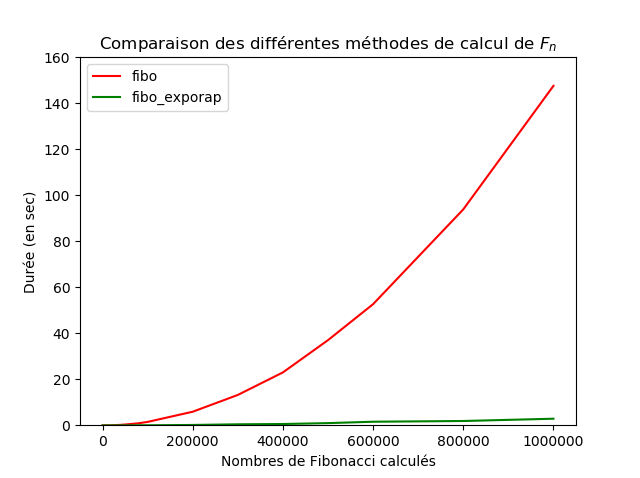
\includegraphics[scale=0.5]{img/Figure.png}
\end{figure}
\end{frame}

\begin{frame}[fragile]
\frametitle{Réponse au problème}
\framesubtitle{Etude comparative}
3 programmes pour calculer les nombres de la suite de Fibonacci :
\begin{itemize}
\item \verb+fibo+
\item \verb+fiborec+ (on l'abandonne car ne satisfait pas les contraintes imposées)
\item \verb+fibo_exporap+ 
\end{itemize}

\begin{alertblock}{Conclusion}
La fonction \verb+fibo_exporap+ (utilisant l'écriture matricielle) est la plus performante dans le calcul des nombres de Fibonacci.
\end{alertblock}
\end{frame}




\begin{frame}
\frametitle{Fin de l'exposé}
\begin{figure}[t]
   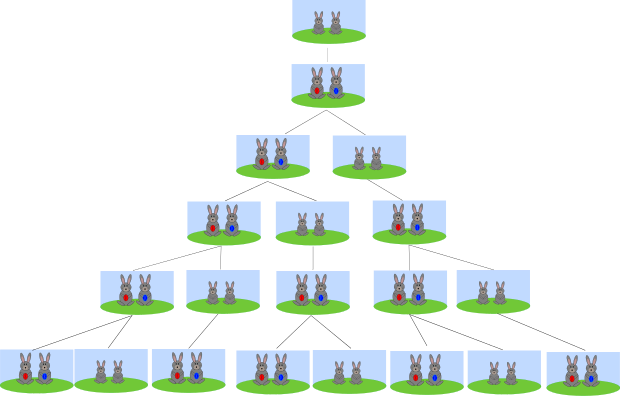
\includegraphics[scale=0.4]{img/Lapins.png}
\end{figure}
\end{frame}
\section*{Annexes}
\begin{frame}[fragile]
\frametitle{Application de Fibonacci : l'algorithme d'Euclide}
\framesubtitle{Définition \& Récursivité}
L'algorithme d'Euclide permet de calculer efficacement le PGCD de 2 nombres entiers $a$ et $b$.
\begin{multicols}{2}
\begin{verbatim}
def euclide(a, b):
    u, v = a, b
    while v != 0:
        r = u % v
        u = v
        v = r
    return u
\end{verbatim}
\columnbreak
\begin{verbatim}
def eucliderec(a, b):
    if b = 0:
        return a
    else:
        return eucliderec(b, a%b)
\end{verbatim}
\end{multicols}
\begin{itemize}
\item \textbf{Cas de base} : $b = 0 \Rightarrow a \wedge b = a$
\item \textbf{Formule de propagation} : $a \wedge b = b \wedge r$
\end{itemize}
\end{frame}

\begin{frame}[fragile]
\frametitle{Application de Fibonacci : l'algorithme d'Euclide}
\framesubtitle{Théorème \& Etude de complexité}
Le théorème de Lamé nous dit que le \textbf{nombre de divisions euclidiennes est inférieur ou égal à 5 fois le nombre de chiffre du plus petit nombre entre $a$ et $b$}.
\pause
\\
De plus, pour calculer $F_{n+2} \wedge F_{n+1}$, \verb+euclide(a,b)+ va effectuer \underline{exactement $n$ divisions} et $F_{n+2} \wedge F_{n+1} = 1$.
\vspace{3mm}
\pause
\begin{alertblock}{Conclusion}
Les nombres de Fibonacci servent de véritables indicateurs dans l'analyse de la complexité de l'algorithme d'Euclide.
\\
Plus précisément, ils permettent d'obtenir une majoration du nombre de divisions euclidiennes et donc de la complexité de ce dernier.
\end{alertblock}
\end{frame}
\end{document}
